\level{2}{Dashboard APS}
	La \insglo{dashboard} è un esempio d'uso di Norris: rappresenta un modo in cui il prodotto può essere utilizzato. Essa, dunque, è una pagina web generata in automatico dal \insglo{server} \insglo{Norris}. Essa è costituita da più grafici che l'utente finale potrà visualizzare sul proprio \insglo{browser}. Di seguito viene fornito un \insglo{mockup} della pagina, che mostra a grandi linee come sarà visualizzata la dashboard una volta completata..
	\begin{figure}[H]\centering
        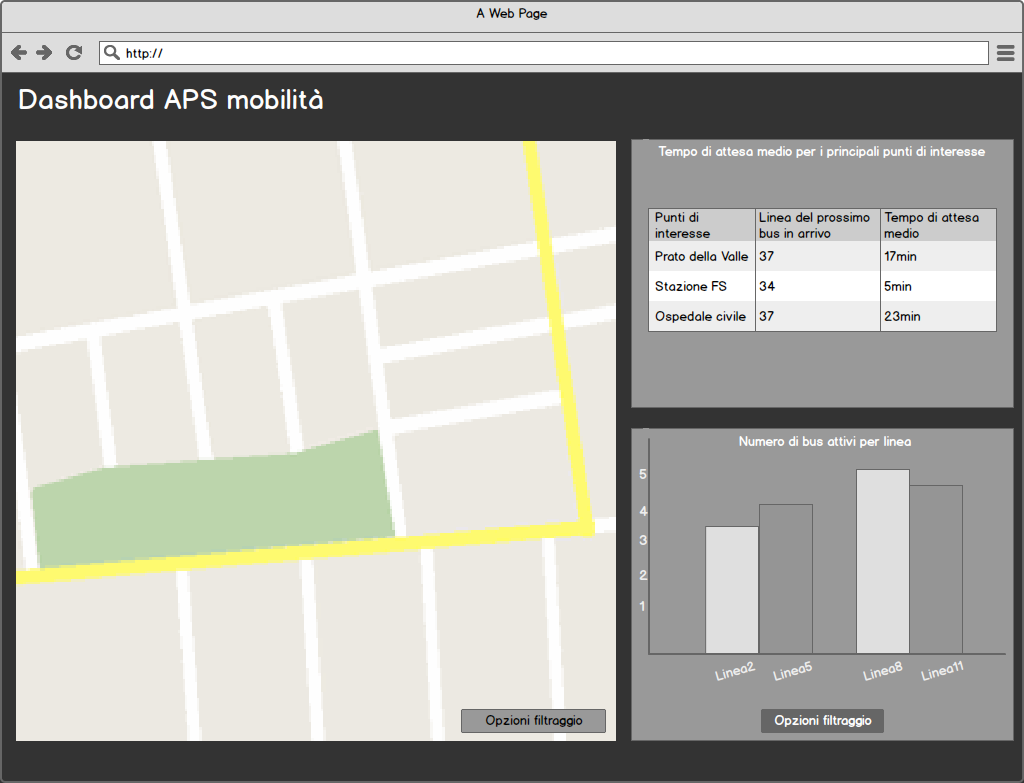
\includegraphics[width=\textwidth]{SpecificaTecnica/Pics/DashboardMockup}
        \caption{Mockup della dashboard APS}
    \end{figure}
    Vengono ora descritti i vari componenti di cui è fatta la pagina, ovvero vengono descritti i grafici che sono stati inseriti all'interno del \insglo{mockup} mostrato in precedenza.
    \level{3}{Descrizione delle componenti della Dashboard}
    	\level{4}{Map chart}
    		Tramite questo grafico l'utilizzatore della \insglo{dashboard} è in grado di visualizzare in tempo reale la posizione di tutti i bus attivi nelle varie linee dell'\insglo{APS}. Tale grafico mette inoltre a disposizione dell'utente delle opzioni riguardanti il filtraggio delle linee presenti: infatti, esso permette di scegliere le linee che si intendono visualizzare, semplicemente nascondendo e ignorando le rimanenti. In questo modo si può trasformare un grafico potenzialmente caotico (a causa della grande quantità di punti presenti al suo interno) in un molto più comprensibile e consultabile.
    	\level{4}{Table}
    		Tale grafico è dedicato ai punti di maggior interesse di Padova. Esso fornisce all'utente utilizzatore della \insglo{dashboard} il tempo necessario all'arrivo degli autobus in alcune fermate \insglo{APS} molto frequentate. In particolare, è possibile visualizzare quanto tempo manca all'arrivo del prossimo autobus in una determinata stazione, e a quale linea il suddetto autobus appartiene. Grazie ad esso gli utenti sono in grado di capire quanto devono attendere mediamente prima di poter salire su uno dei mezzi da loro scelti.
    	\level{4}{Bar chart}
    		Questo grafico permette all'utilizzatore della \insglo{dashboard} di visualizzare quanti autobus sono attivi su ciascuna linea dell'\insglo{APS}. Tale grafico mette inoltre a disposizione dell'utente delle opzioni riguardanti il filtraggio delle linee presenti: infatti, esso permette di scegliere le linee di cui si vuole visualizzare il numero di bus attivi. Grazie a questo grafico, l'utente può ottenere utili informazioni su quanto una linea è frequentata e sul tempo di attesa che mediamente passa tra làarrivo di un mezzo e del successivo.